% Schema
\section{Userspace}
	\begin{frame}
		\begin{figure}
		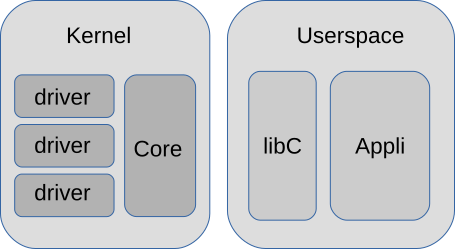
\includegraphics[height=4cm]{img/arch_linux_full.png}
		\caption{kernel + userspace}
		\end{figure}
	\end{frame}

	\begin{frame}
		\center{\huge{Rootfs}}
		\begin{block}<2->{Librairies}
			\begin{itemize}
				\item libC : GNU libC, uClibC, dietlibC
				\item librairies métier
			\end{itemize}
		\end{block}
		\begin{block}<3->{Utilitaires}
			\begin{itemize}
				\item Commandes standard : GNU Coreutils, Busybox
				\item Applications métier
				\item Daemons système
			\end{itemize}
		\end{block}
	\end{frame}
	\begin{frame}
		\center{\huge{Système d'init}}
		\begin{itemize}
			\item<1-> Premier processus lancé
			\item<2-> Lance les autres processus
			\item<3-> Influe sur le temps de boot
		\end{itemize}
		\begin{columns}[t]
			\begin{column}{0.48\textwidth}
				\begin{block}<4->{SysV init}
					\begin{itemize}
						\item Scripts
						\item Peu de parallélisation
						\item Simple
					\end{itemize}
				\end{block}
			\end{column}
			\begin{column}{0.48\textwidth}
				\begin{block}<5->{Systemd}
					\begin{itemize}
						\item Fichiers de configuration
						\item Parallélisation
						\item Plus complexe
					\end{itemize}
				\end{block}
			\end{column}
		\end{columns}
	\end{frame}

